% Created 2018-10-25 jue 16:29
% Intended LaTeX compiler: pdflatex
\documentclass[xcolor={usenames,svgnames,dvipsnames}]{beamer}
\usepackage[utf8]{inputenc}
\usepackage[T1]{fontenc}
\usepackage{graphicx}
\usepackage{grffile}
\usepackage{longtable}
\usepackage{wrapfig}
\usepackage{rotating}
\usepackage[normalem]{ulem}
\usepackage{amsmath}
\usepackage{textcomp}
\usepackage{amssymb}
\usepackage{capt-of}
\usepackage{hyperref}
\usepackage{color}
\usepackage{listings}
\usepackage{mathpazo}
\usepackage{gensymb}
\usepackage{amsmath}
\usepackage{chemarr}%flechas para reacciones químicas (SFER.tex)
\bibliographystyle{plain}
\AtBeginSubsection[]{\begin{frame}[plain]\tableofcontents[currentsubsection,sectionstyle=show/shaded,subsectionstyle=show/shaded/hide]\end{frame}}
\AtBeginSection[]{\begin{frame}[plain]\tableofcontents[currentsection,hideallsubsections]\end{frame}}
\usepackage[emulate=units]{siunitx}
\sisetup{fraction=nice, decimalsymbol=comma, retain-unity-mantissa = false}
\newunit{\wattpeak}{Wp}
\newunit{\watthour}{Wh}
\newunit{\amperehour}{Ah}
\usepackage{steinmetz}
\hypersetup{colorlinks=true, linkcolor=Blue, urlcolor=Blue}
\renewcommand{\thefootnote}{\fnsymbol{footnote}}
\beamertemplatenavigationsymbolsempty
\setbeamertemplate{footline}[frame number]
\setbeamercolor{alerted text}{fg=blue!50!black} \setbeamerfont{alerted text}{series=\bfseries}
\usetheme[hideothersubsections]{Goettingen}
\usecolortheme{rose}
\usefonttheme{serif}
\author{Oscar Perpiñán Lamigueiro}
\date{\url{http://oscarperpinan.github.io}}
\title{Máquinas Eléctricas \\ Aparamenta Eléctrica}
\hypersetup{
 pdfauthor={Oscar Perpiñán Lamigueiro},
 pdftitle={Máquinas Eléctricas \\ Aparamenta Eléctrica},
 pdfkeywords={},
 pdfsubject={},
 pdfcreator={Emacs 25.2.2 (Org mode 9.1.13)}, 
 pdflang={Spanish}}
\begin{document}

\maketitle

\section{Fundamentos de Electromagnetismo}
\label{sec:orgb470ab8}

\begin{frame}[label={sec:org5135053}]{Fuerza Magnética}
Un campo magnético ejerce una fuerza sobre una carga en movimiento (o corriente eléctrica en un conductor) \footnote{Fuerza de Lorentz}.
\[
\vec{F} = q (\vec{v} \times \vec{B})
\]

\begin{columns}
\begin{column}{0.5\columnwidth}
\begin{center}
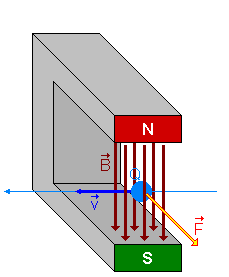
\includegraphics[height=0.5\textheight]{../figs/Fuerza_Lorentz.png}
\end{center}
\end{column}

\begin{column}{0.5\columnwidth}
\begin{center}
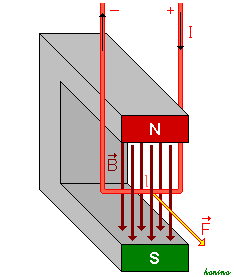
\includegraphics[height=0.5\textheight]{../figs/Fuerza_Lorentz_Conductor.png}
\end{center}
\end{column}
\end{columns}
\end{frame}

\begin{frame}[label={sec:org508b5fa}]{Campo Magnético creado por un Conductor}
Una corriente eléctrica crea un campo magnético en torno al conductor\footnote{Ley de Biot-Savart (y Oersted). Ley de Ampere.}. 

\begin{columns}
\begin{column}{0.5\columnwidth}
\begin{center}
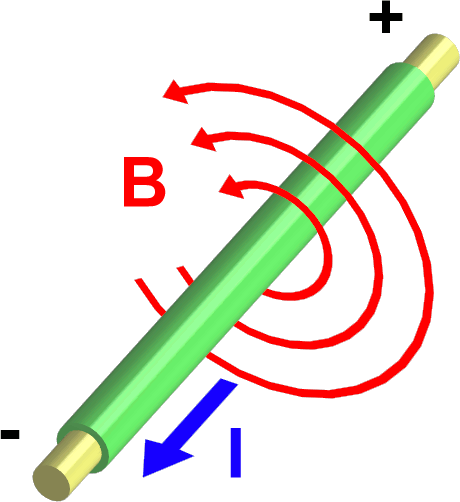
\includegraphics[width=.9\linewidth]{../figs/Electromagnetism.png}
\end{center}
\end{column}
\begin{column}{0.5\columnwidth}
\begin{center}
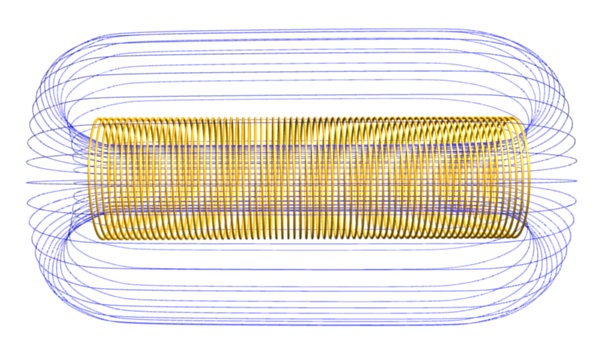
\includegraphics[width=.9\linewidth]{../figs/Solenoide.jpg}
\end{center}
\end{column}
\end{columns}
\end{frame}

\begin{frame}[label={sec:org9cb6e55}]{Interacción entre Conductores}
Dos conductores se repelen o atraen según el sentido de sus corrientes.

\begin{center}
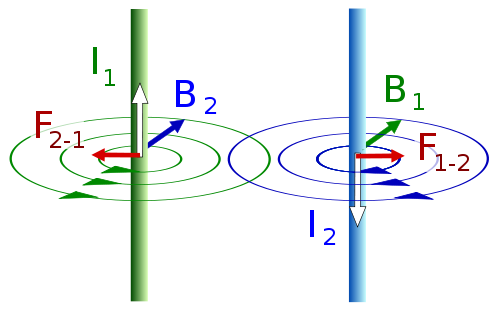
\includegraphics[width=.9\linewidth]{../figs/FuerzasRepulsion.png}
\end{center}
\begin{center}
Vídeo: \href{https://www.youtube.com/watch?v=2j8D\_N1v0tU\&t=0m15s}{Repulsión entre barras de Alta Tensión}
\end{center}
\end{frame}
\begin{frame}[label={sec:org06d034e}]{Flujo Magnético}
El flujo magnético es la cantidad de líneas de fuerza magnética que atraviesan una superficie. 

Depende de la densidad de campo, \(B\), el área de la superficie, \(A\), y la posición relativa entre ambos, \(\theta\).

\[
\phi = B \cdot A \cdot \cos \theta
\]

\begin{center}
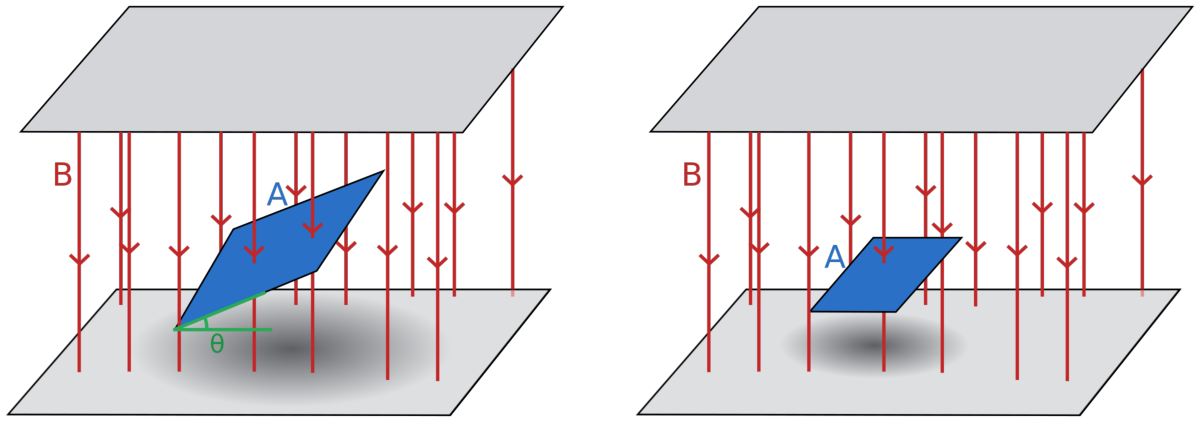
\includegraphics[width=.9\linewidth]{../figs/flujo_magnetico.pdf}
\end{center}
\end{frame}

\begin{frame}[label={sec:org4537cbd}]{Ley de Faraday}
\begin{itemize}
\item Cuando el \alert{flujo magnético} que atraviesa una espira es \alert{variable}
aparece \alert{tensión inducida}.
\end{itemize}

\[
e=- N \frac{\mathrm{d}\phi}{\mathrm{d}t} = - N \frac{\mathrm{d}(B \cdot S\cdot \cos \theta)}{\mathrm{d}t} 
\]

\begin{itemize}
\item El flujo es variable cuando:

\begin{itemize}
\item La \alert{espira está en movimiento} (\(\theta\))

\item El \alert{campo magnético \(B\) es variable},

\item Ambas situaciones coinciden.
\end{itemize}

\item La tensión inducida es directamente proporcional a la rapidez de la
variación.
\end{itemize}
\end{frame}


\section{Máquinas Eléctricas}
\label{sec:org3ae8fb1}
\subsection{Introducción}
\label{sec:org36d0c13}

\begin{frame}[label={sec:org1d4eeea}]{Máquina Eléctrica}
Una máquina eléctrica realiza una conversión entre dos formas de energía, una de ellas eléctrica:

\begin{itemize}
\item \alert{Motor}: transforma la energía eléctrica en energía mecánica.
\item \alert{Generador}: transforma la energía mecánica en energía eléctrica.
\item \alert{Transformador}: transforma las condiciones (tensión y corriente) de la energía eléctrica de entrada en otras diferentes de salida.
\end{itemize}
\end{frame}

\begin{frame}[label={sec:orgf019ade}]{Partes de una Máquina}
\begin{columns}
\begin{column}{0.5\columnwidth}
\begin{itemize}
\item \alert{Estátor}: parte fija de forma cilíndrica.
\item \alert{Rótor}: parte giratoria situada en la cavidad del estátor.
\item \alert{Entrehierro}: espacio de aire que separa el estátor del rótor.
\end{itemize}
\end{column}
\begin{column}{0.5\columnwidth}
\begin{center}
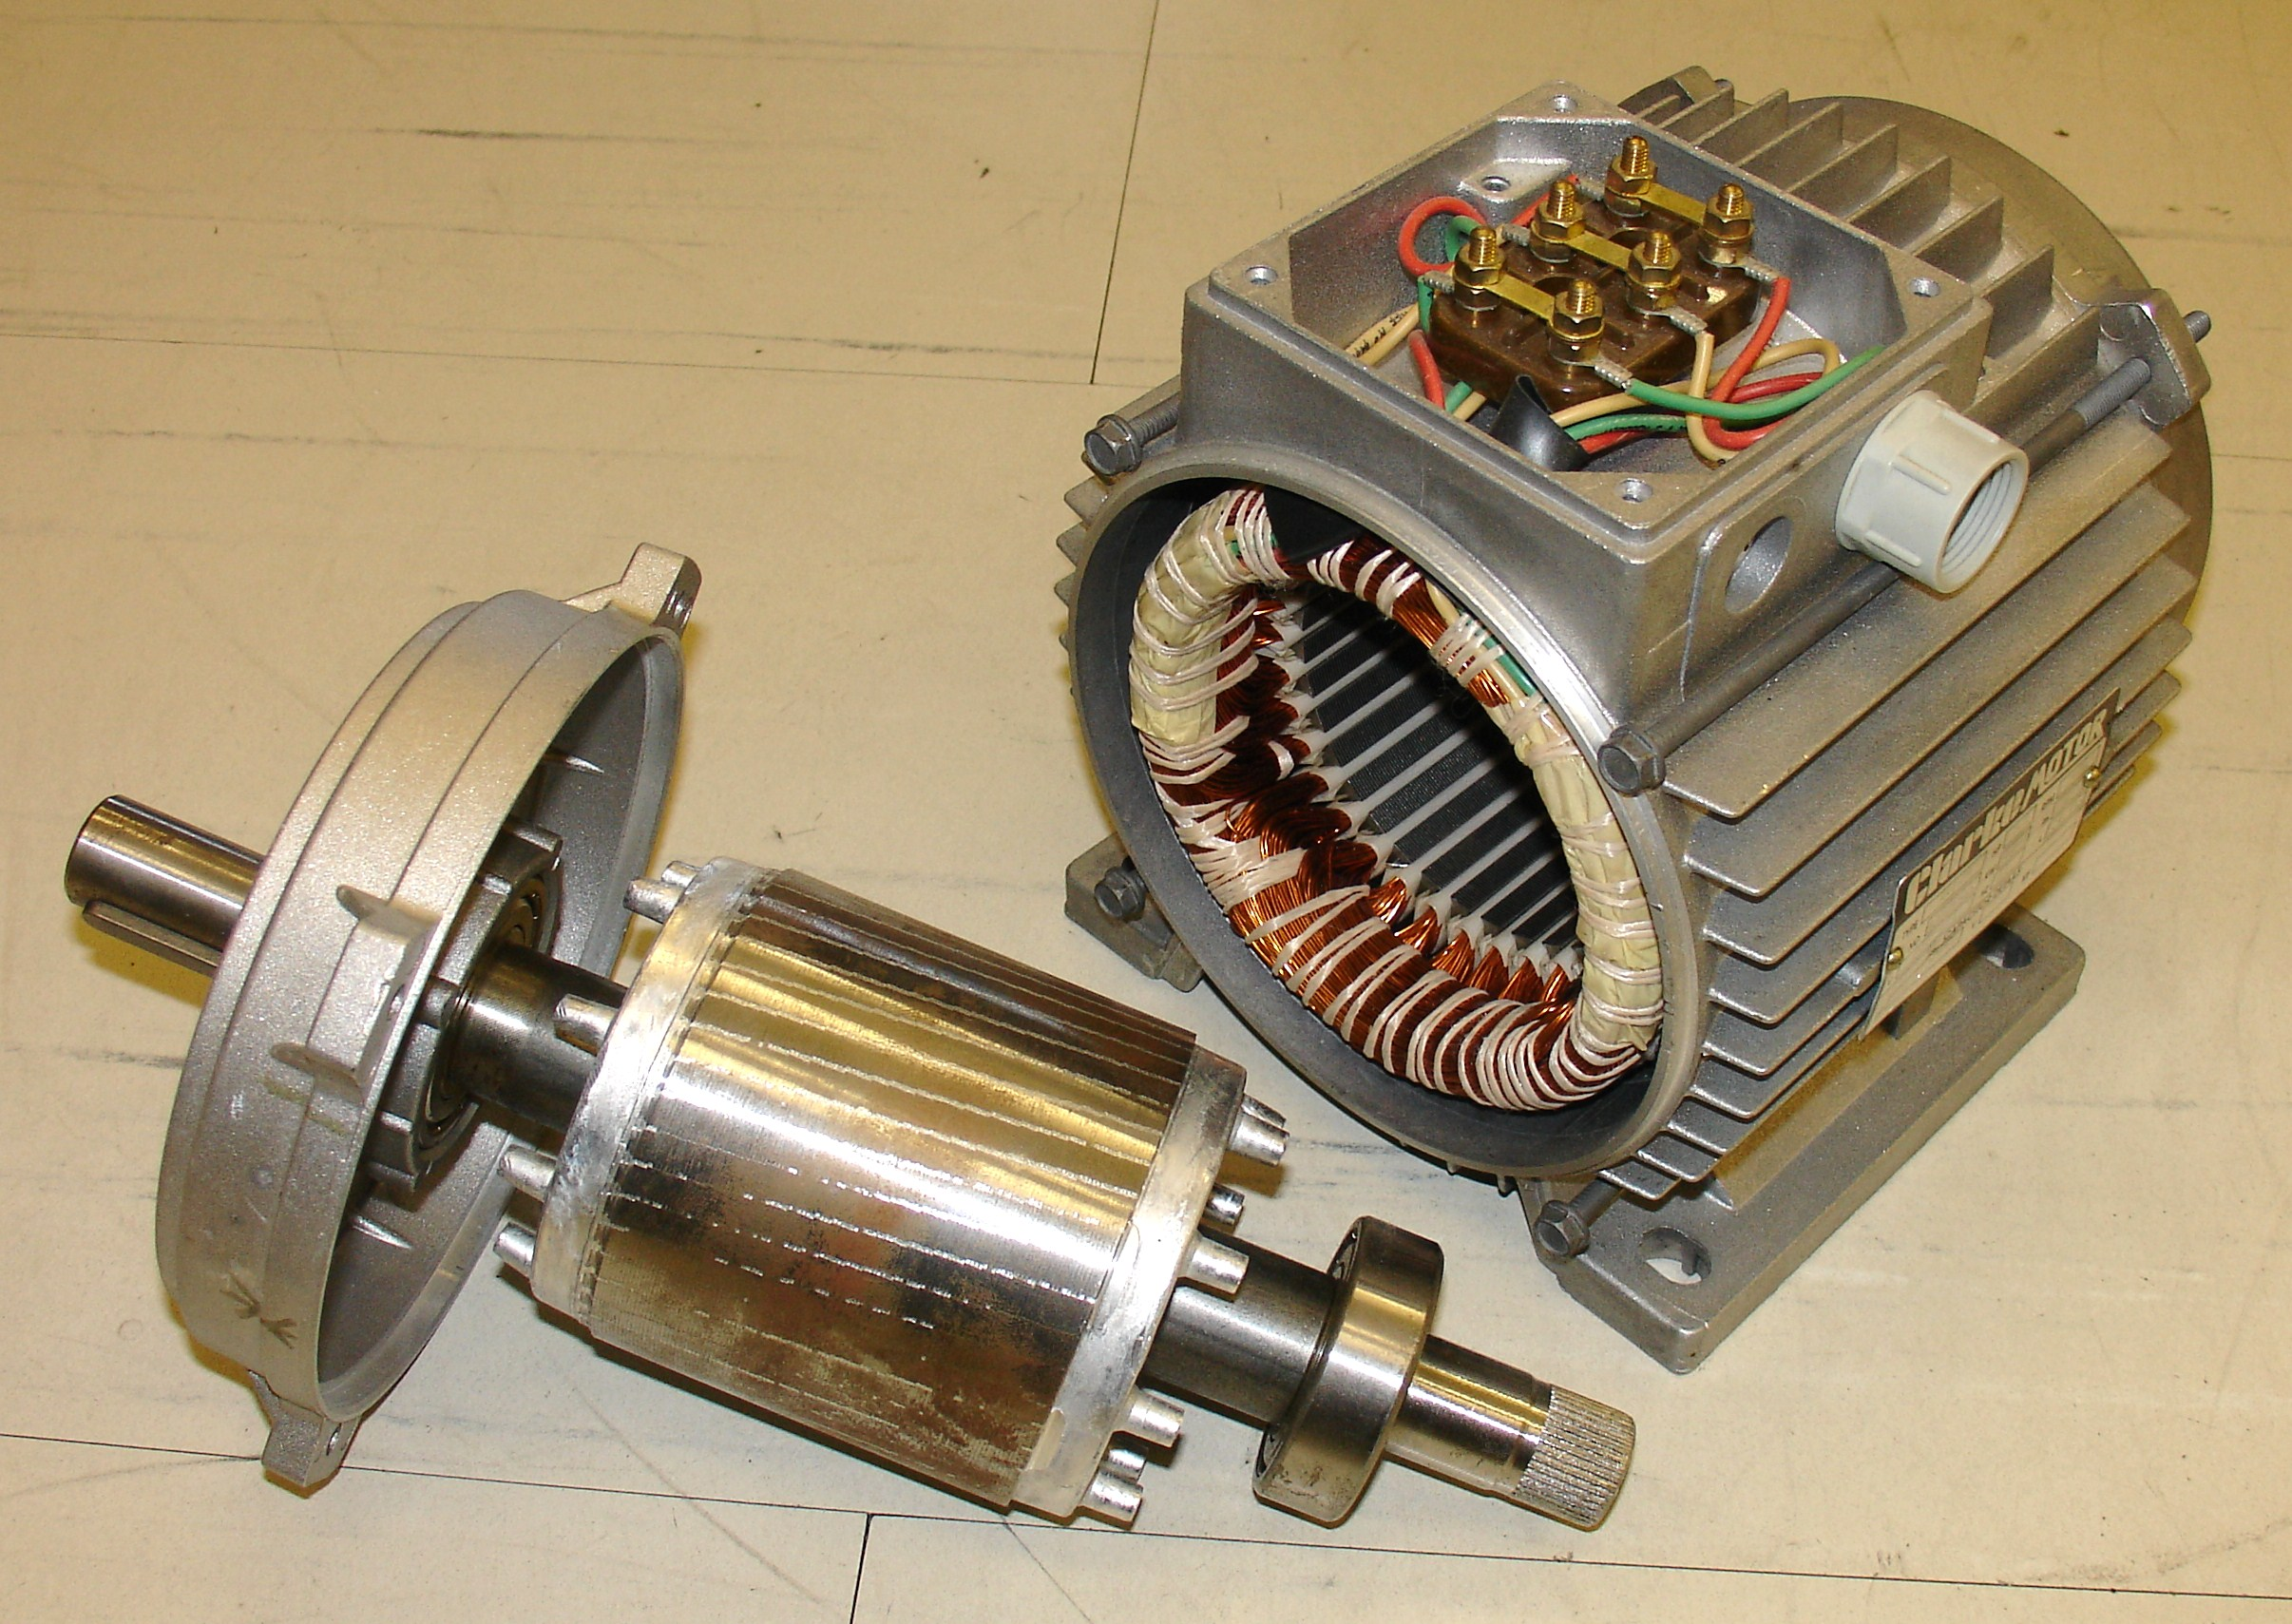
\includegraphics[width=.9\linewidth]{../figs/Stator_and_rotor_by_Zureks.jpeg}
\end{center}
\end{column}
\end{columns}

\begin{block}{}
La transformación de energía eléctrica y mecánica se produce a través del campo magnético del entrehierro, lugar del acoplamiento energético entre estátor y rótor. 
\end{block}
\end{frame}

\begin{frame}[label={sec:org613bf83}]{Inductor e Inducido}
Al elemento que emite el campo magnético se le denomina \alert{inductor} y aquel que es atravesado por este flujo es el \alert{inducido}.
\begin{center}
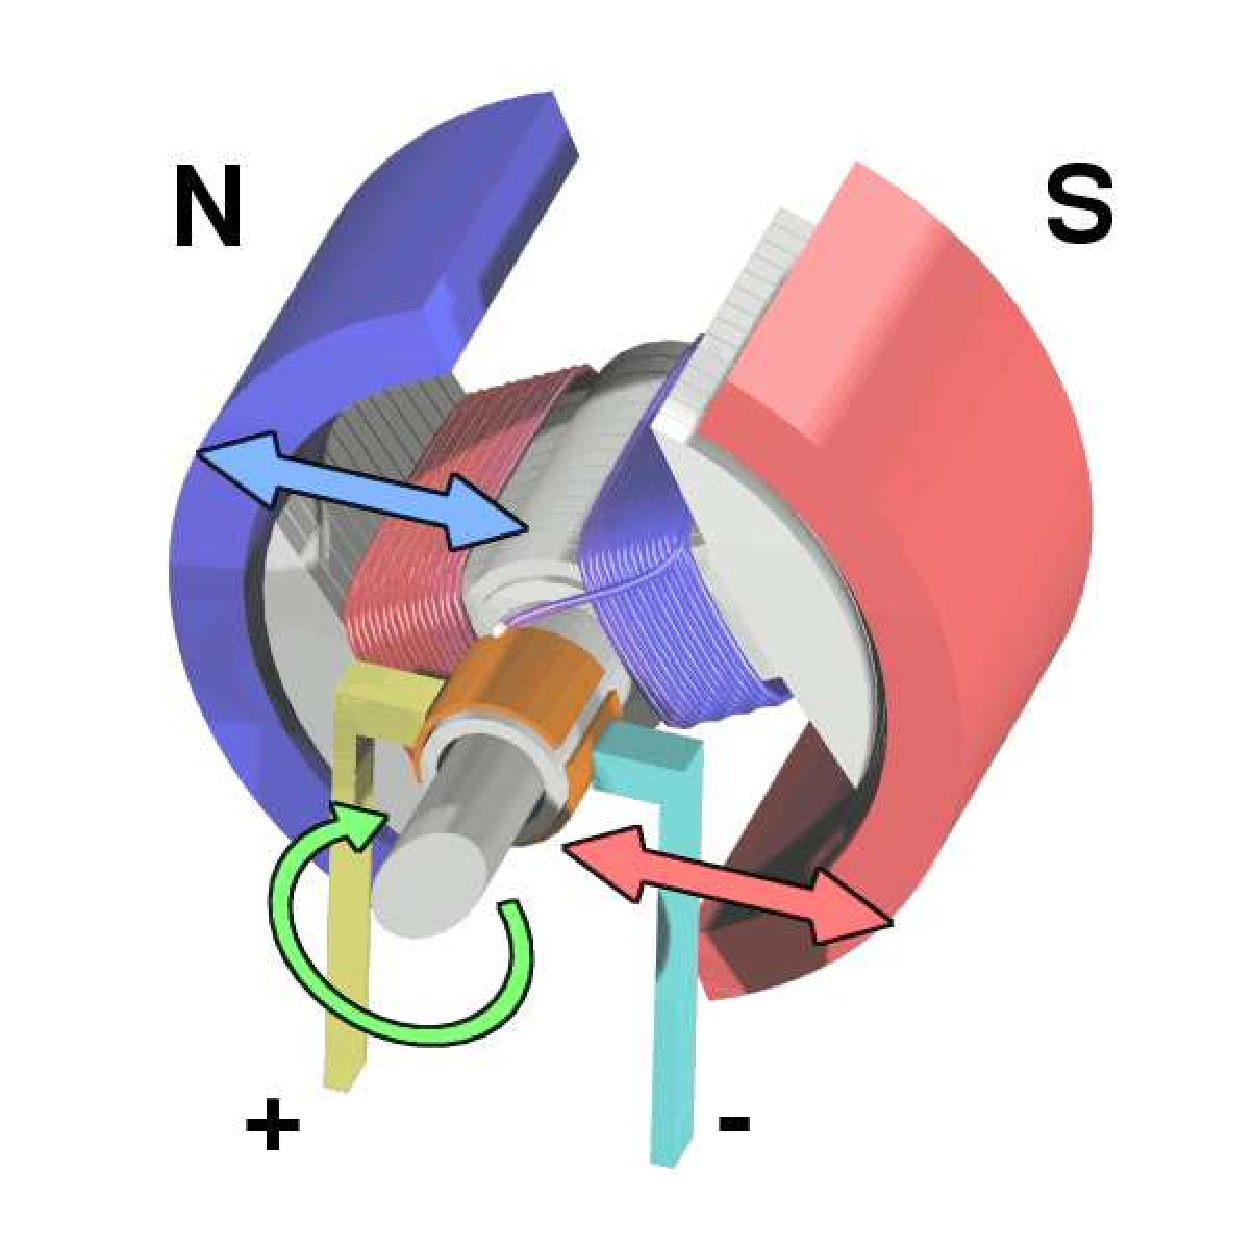
\includegraphics[height=0.5\textheight]{../figs/Electric_motor_cycle_3.pdf}
\end{center}
\end{frame}

\subsection{Tipos de Máquinas}
\label{sec:org6a30912}

\begin{frame}[label={sec:org03e9873}]{Motor}
\begin{itemize}
\item La energía eléctrica de entrada produce una corriente eléctrica que genera un campo magnético variable.
\item Este campo puede interactuar con otro campo magnético existente o con otro conductor y produce movimiento.
\item Más habituales: de inducción, y de corriente continua.
\end{itemize}
\end{frame}


\begin{frame}[label={sec:org4e8b5a8}]{Motor asíncrono o de inducción}
\begin{itemize}
\item Estator-Inductor alimentado por una corriente trifásica alterna (campo giratorio)

\item Rotor-Inducido constituido por espiras cortocircuitadas (jaula de
ardilla).

\item Rotor gira a menor velocidad que el campo.
\end{itemize}

\begin{center}
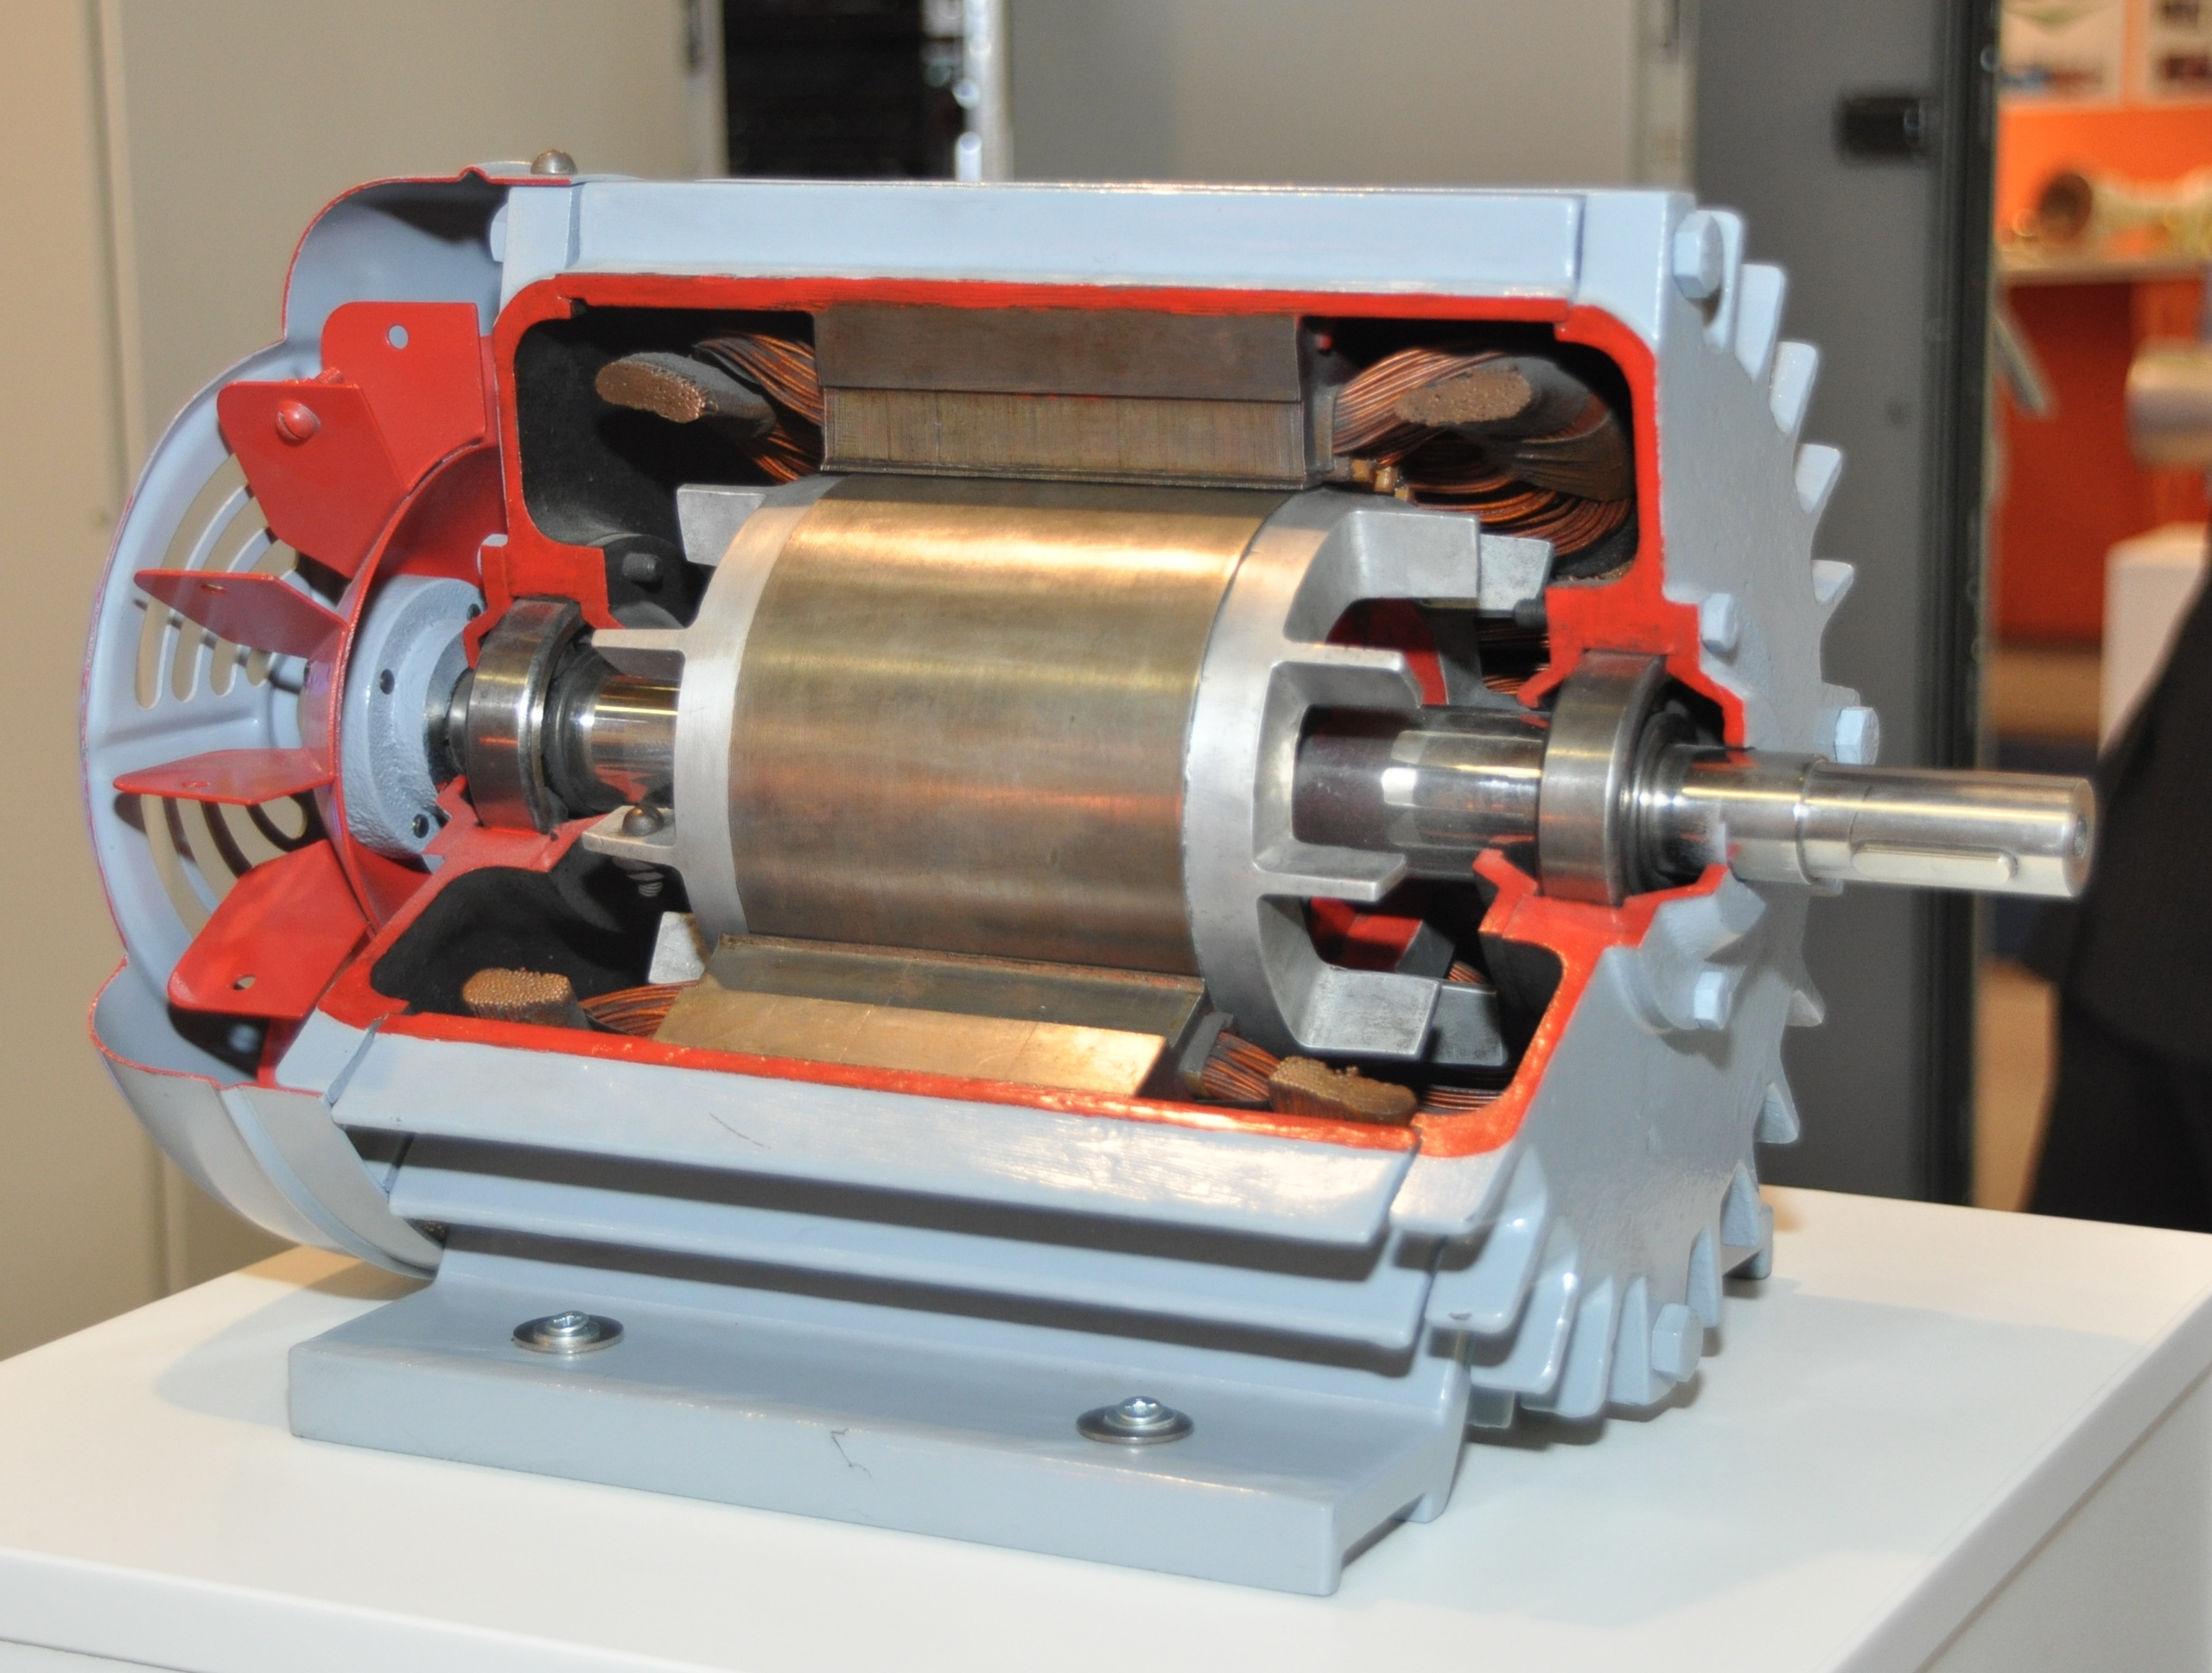
\includegraphics[height=0.5\textheight]{../figs/Seccion_Motor.jpeg}
\end{center}

Vídeos: Motor de inducción artesanal \href{http://www.youtube.com/watch?v=ZRGlAu0uCHY\&feature=related}{(1)} \href{http://www.youtube.com/watch?v=P-eTLmJC2cQ}{(2)}
\end{frame}

\begin{frame}[label={sec:org9376822}]{Motor DC}
\begin{itemize}
\item Estator-Inductor con imanes permanentes o alimentado por corriente DC.

\item Rotor-Inducido alimentado con corriente DC a través de un colector de delgas, o sin escobillas.
\end{itemize}

\begin{center}
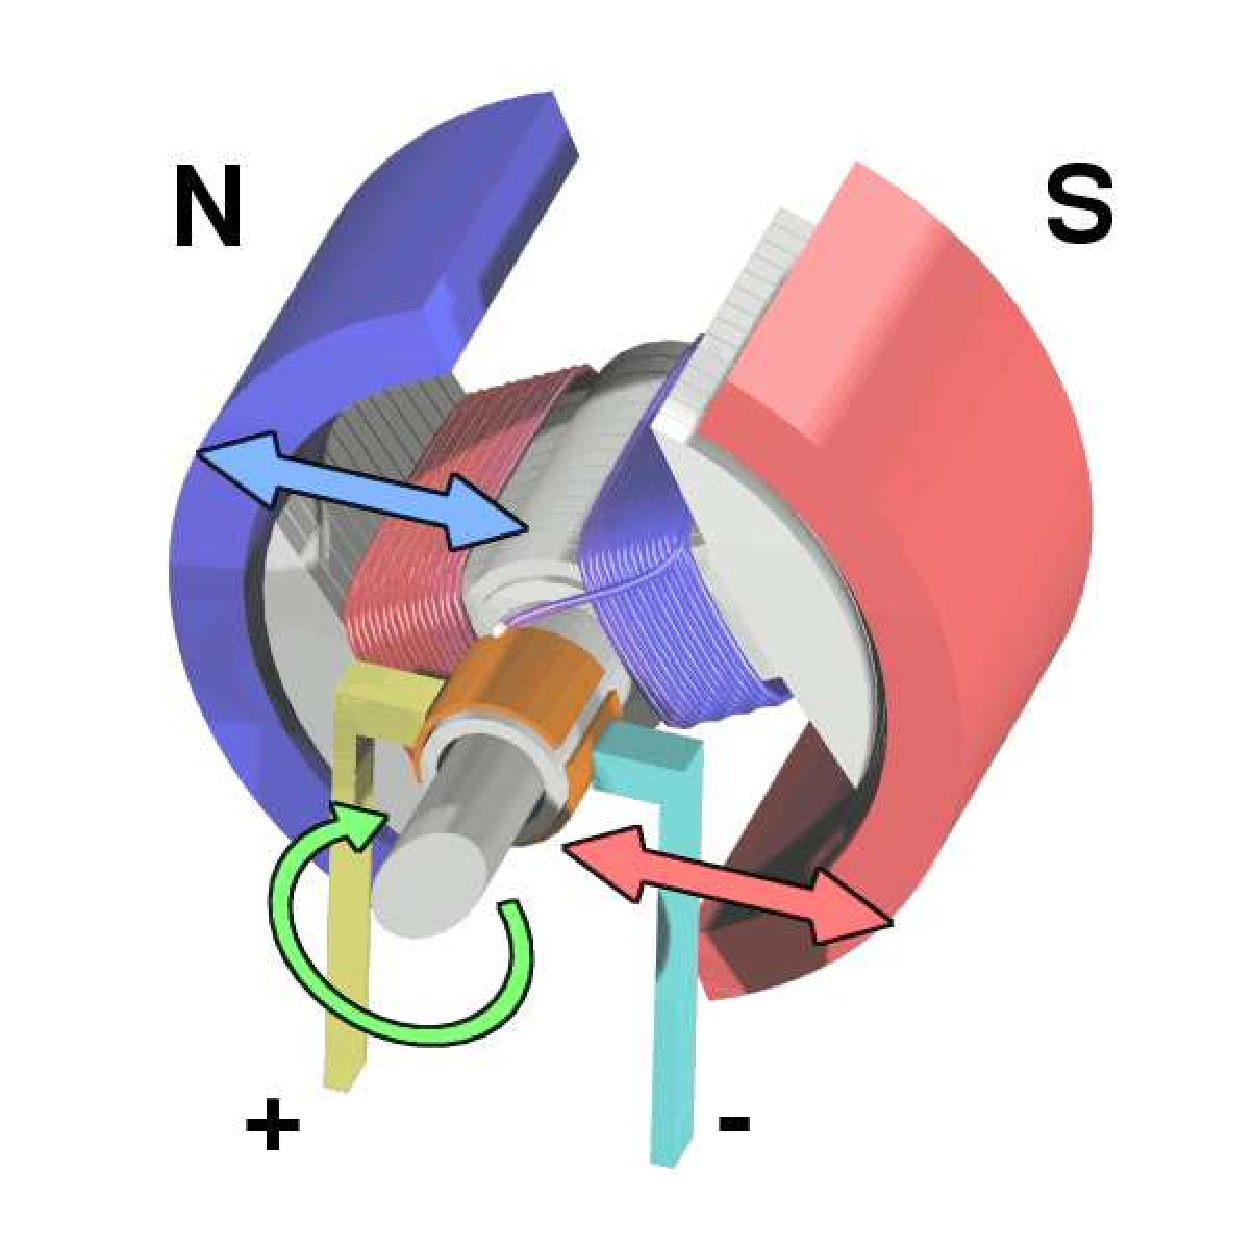
\includegraphics[height=0.6\textheight]{../figs/Electric_motor_cycle_3.pdf}
\end{center}
\end{frame}


\begin{frame}[label={sec:org0b4752c}]{Generador}
\begin{itemize}
\item Existe un campo magnético en el interior de la máquina (p. ej. imanes permanentes)
\item La energía mecánica de entrada aporta movimiento a una bobina en el seno del campo.
\item La interacción entre el campo y las espiras de la bobina producen una tensión inducida.
\item Más habituales: asíncrono, síncrono, y de corriente continua.
\end{itemize}
\end{frame}

\begin{frame}[label={sec:org4307221}]{Generador Asíncrono}
\begin{columns}
\begin{column}{0.6\columnwidth}
\begin{itemize}
\item Estator-Inductor alimentado por una corriente trifásica alterna (campo giratorio)

\item Rotor-Inducido constituido por espiras cortocircuitadas (jaula de
ardilla).

\item Rotor debe girar a mayor velocidad que la del campo del estator.

\item Empleado en turbinas eólicas
\end{itemize}
\end{column}
\begin{column}{0.5\columnwidth}
\begin{center}
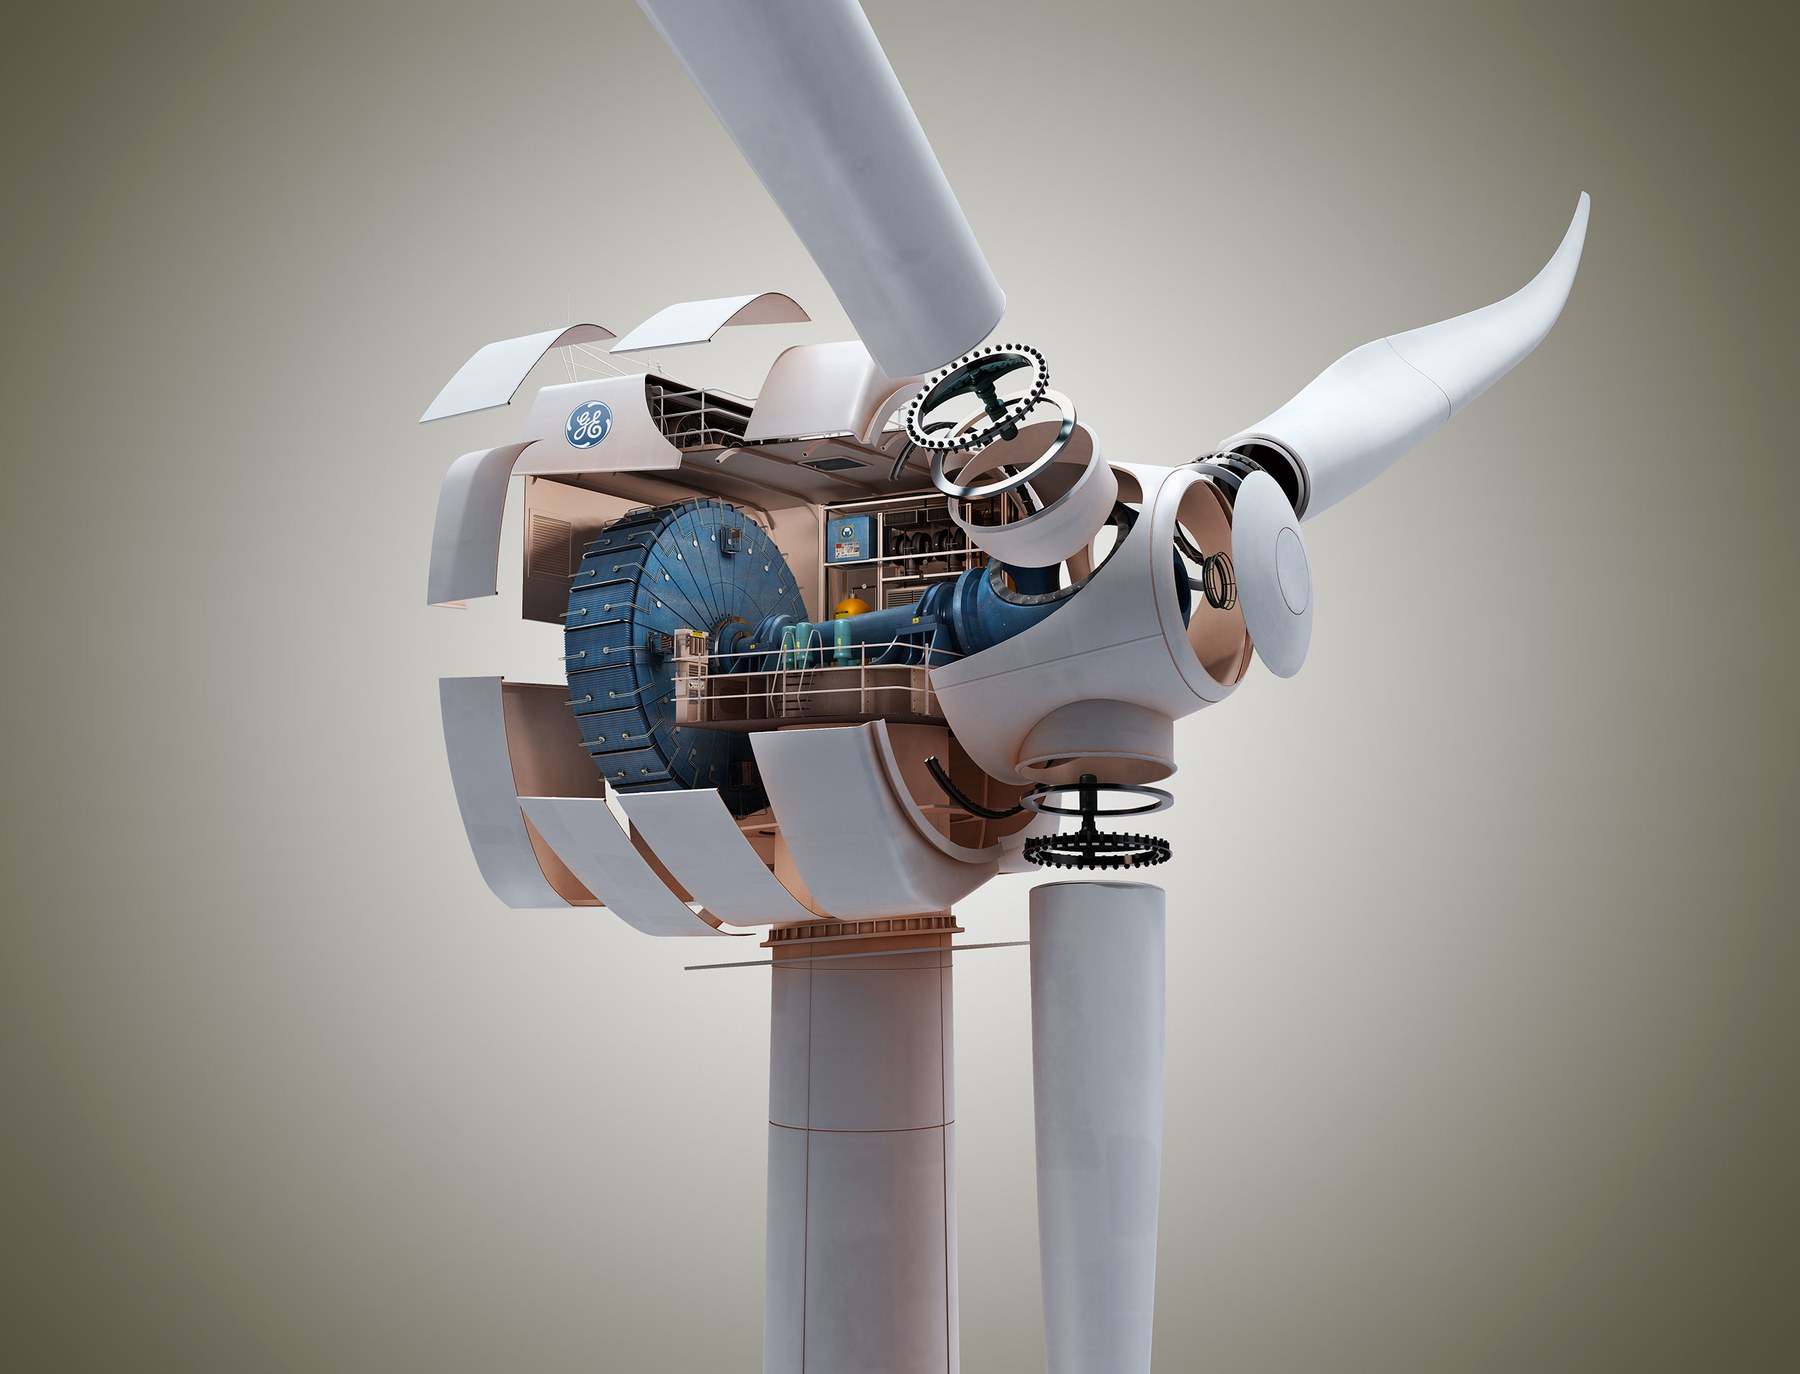
\includegraphics[width=.9\linewidth]{../figs/InsideWindTurbine.jpg}
\end{center}
\end{column}
\end{columns}
\end{frame}

\begin{frame}[label={sec:org6c62a42}]{Generador Síncrono o Alternador}
\begin{itemize}
\item Rotor-inductor alimentado por corriente continua mediante anillos.

\item Estator-inducido constituido por un devanado trifásico.

\item Velocidad de giro constante, sincronizada con la frecuencia de red.

\item Empleado en turbinas hidráulicas y térmicas.
\end{itemize}
\end{frame}

\begin{frame}[label={sec:org0145af6}]{Generador DC}
\begin{itemize}
\item Estator-Inductor alimentado por corriente DC (o imanes permanentes).

\item El colector de delgas transforma la frecuencia de alimentación (DC)
en alterna.

\item Empleado en máquinas eólicas de baja potencia.
\end{itemize}
\end{frame}


\begin{frame}[label={sec:orgdee8163}]{Transformador}
\begin{columns}
\begin{column}{0.6\columnwidth}
\begin{itemize}
\item La energía eléctrica de entrada alimenta una bobina con un número de espiras \(N_p\).
\item El campo magnético generado por esta bobina circula hasta una bobina de salida, con \(N_s\) espiras.
\item El diferente número de espiras provoca valores de tensión y corriente diferente en la entrada y salida.
\end{itemize}
\end{column}

\begin{column}{0.4\columnwidth}
\begin{center}
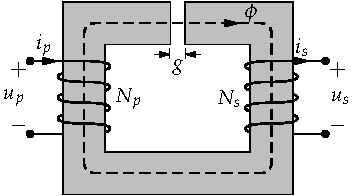
\includegraphics[width=.9\linewidth]{../figs/Transformador2.pdf}
\end{center}
\begin{center}
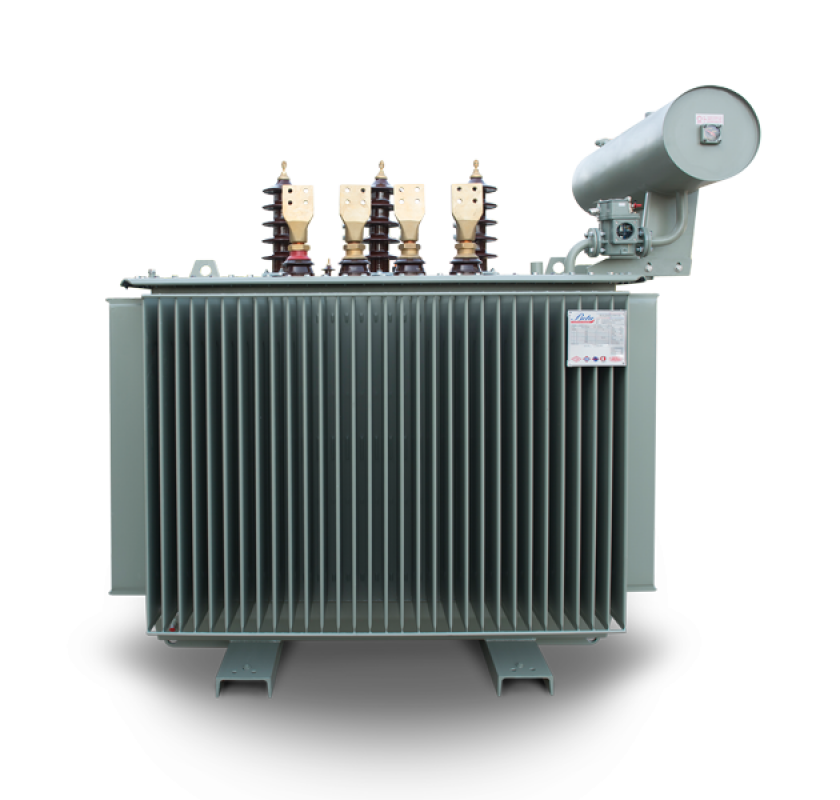
\includegraphics[width=.9\linewidth]{../figs/Transformador.png}
\end{center}
\end{column}
\end{columns}
\end{frame}

\begin{frame}[label={sec:org020d9c4}]{Transformador}
\begin{align*}
N_{s}\cdot I_{s} &= N_{p}\cdot I_{p}\\
\frac{V_{p}}{N_{p}} &= \frac{V_{s}}{N_{s}}
\end{align*}

\begin{center}
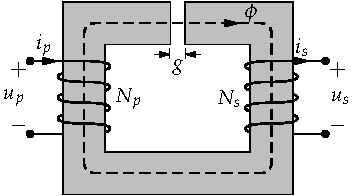
\includegraphics[height=0.3\textheight]{../figs/Transformador2.pdf}
\end{center}

\begin{itemize}
\item Ejemplo: un transformador elevador sube tensión (\(V_{s}>V_{p}\)) y reduce corriente (\(I_{s}<I_{p}\)): \(N_{p}/N_{s}<1\), más vueltas en el secundario que en el primario.
\end{itemize}
\end{frame}


\section{Aparamenta eléctrica}
\label{sec:org51e4688}

\subsection{Sistema de Suministro Eléctrico}
\label{sec:org0e18c9f}
\begin{frame}[label={sec:org2a45656}]{Sistema de suministro eléctrico}
Un \alert{sistema de suministro eléctrico} tiene como objetivo \alert{producir,
transportar y distribuir energía eléctrica} a los lugares de consumo,
con el mínimo coste posible en condiciones de \alert{fiabilidad, calidad y
seguridad}.
\end{frame}

\begin{frame}[label={sec:org0685a36}]{Componentes del Sistema de Suministro Eléctrico}
\begin{center}
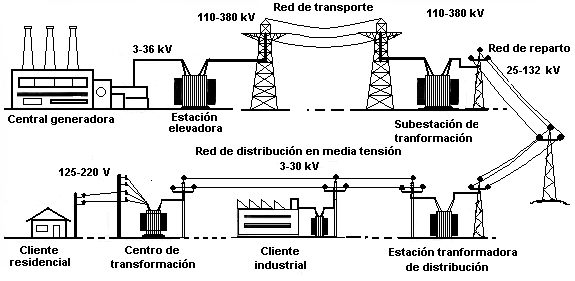
\includegraphics[width=.9\linewidth]{../figs/Redelectrica2.png}
\end{center}

\begin{itemize}
\item Generadores

\item Redes de transporte

\item Redes de distribución

\item Equipos de acondicionamiento, transformación y protección (y en
algunos casos, almacenamiento)

\item Puntos de consumo
\end{itemize}
\end{frame}


\subsection{Definición y Funciones}
\label{sec:org7f1e26d}
\begin{frame}[label={sec:org6ae8904}]{Definición}
\begin{block}{ITC-BT-01}
\begin{description}
\item[{Aparamenta:}] Equipo, aparato o material previsto para ser conectado a un circuito eléctrico con el fin de asegurar una o varias de las siguientes funciones: \alert{protección}, \alert{control}, \alert{seccionamiento}, \alert{conexión}.

\item[{Función de la Aparamenta:}] Garantizar la seguridad de las personas,
la continuidad en el suministro y la protección de los elemento de la
instalación.
\end{description}
\end{block}
\end{frame}

\begin{frame}[label={sec:org13a5ec6}]{Funciones de la aparamenta}
\begin{itemize}
\item \alert{Protección}:

\begin{itemize}
\item Protección de los elementos de los circuitos contra las tensiones
térmicas y mecánicas de las corrientes de cortocircuito.

\item Protección de las personas en caso de producirse un defecto de
aislamiento.

\item Protección de los dispositivos y aparatos suministrados.
\end{itemize}
\end{itemize}
\end{frame}

\begin{frame}[label={sec:orge64effb}]{Funciones de la aparamenta}
\begin{itemize}
\item \alert{Aislamiento}: separar de forma verificable un circuito, un aparato o
un elemento de la planta del resto de un sistema que se encuentra en
tensión, con el fin de que el personal pueda realizar con total
seguridad trabajos en la parte aislada.
\end{itemize}
\end{frame}

\begin{frame}[label={sec:org2ccda90}]{Funciones de la aparamenta}
\begin{itemize}
\item \alert{Control:} modificar un sistema cargado en cualquier momento

\begin{itemize}
\item Control funcional (conmutación rutinaria, etc.).

\item Conmutación de emergencia.

\item Operaciones de mantenimiento del sistema de alimentación.
\end{itemize}
\end{itemize}
\end{frame}

\begin{frame}[label={sec:org772f630}]{Arco Eléctrico}
\begin{itemize}
\item Descarga eléctrica que se forma entre dos electrodos sometidos a una diferencia de potencial.
\item Durante el tiempo de la descarga se produce una luminosidad muy intensa y un gran desprendimiento de calor.
\item Ambos fenómenos, en caso de ser accidentales, pueden ser sumamente destructivos.
\end{itemize}

\begin{center}
Vídeo: \href{http://www.youtube.com/watch?v=WBTvGqRA4\_0}{Apertura en Alta Tensión}
\end{center}
\end{frame}

\begin{frame}[label={sec:org8a61c30}]{Poder de corte y cierre}
\begin{description}
\item[{Poder de corte:}] intensidad de corriente que este dispositivo es
capaz de cortar, bajo una tensión de restablecimiento determinada.

\item[{Poder de cierre:}] intensidad de corriente que este aparato es capaz
de establecer, bajo una tensión dada.
\end{description}
\end{frame}

\subsection{Tipos de Dispositivos}
\label{sec:org39b1466}
\begin{frame}[label={sec:orgee14664}]{Dispositivos simples}
\begin{block}{Seccionador}
\begin{itemize}
\item Dispositivo de dos posiciones (abierto/cerrado) enclavable y accionado manualmente que proporciona un aislamiento seguro de un circuito cuando está enclavado en la posición abierta.

\item Un seccionador no está diseñado para abrir o cerrar el paso de la corriente.
\end{itemize}
\end{block}

\begin{block}{Interruptor de carga}
\begin{itemize}
\item Dispositivo no automático (accionamiento manual) de dos posiciones (abierto/cerrado).
\item Se utiliza para cerrar y abrir circuitos cargados en condiciones normales de circuitos sin defectos.
\end{itemize}
\end{block}
\end{frame}

\begin{frame}[label={sec:org76afdba}]{Dispositivos simples}
\begin{block}{Contactor}
\begin{itemize}
\item Dispositivo accionado por solenoide que por lo general se mantiene cerrado mediante una corriente (reducida).

\item Se suelen controlar de forma remota por medio de pulsadores de activación/desactivación.
\end{itemize}
\end{block}

\begin{block}{Fusible}
\begin{itemize}
\item Un filamento o lámina de un metal o aleación de bajo punto de fusión que se intercala en un punto determinado de una instalación eléctrica

\item Se funde por Efecto Joule cuando la intensidad de corriente supere, por un cortocircuito o un exceso de carga.

\item Es capaz de abrir un circuito en carga.
\end{itemize}
\end{block}
\end{frame}

\begin{frame}[label={sec:org507513b}]{Interruptor magnetotérmico}
\begin{itemize}
\item Dispositivo automático capaz de interrumpir la corriente eléctrica de un circuito cuando ésta sobrepasa ciertos valores máximos.

\item El dispositivo consta de dos partes, un electroimán y una lámina bimetálica, conectadas en serie y por las que circula la corriente que va hacia la carga.

\item Su funcionamiento se basa en dos de los efectos producidos por la circulación de corriente eléctrica en un circuito: el magnético y el térmico (efecto Joule).

\item Se emplea para \alert{proteger contra sobreintensidades y sobrecargas}.
\end{itemize}

\begin{center}
Vídeo: \href{http://www.youtube.com/watch?v=c6QqnLgWbCQ}{Apertura de un PIA}
\end{center}
\end{frame}

\begin{frame}[label={sec:org50147e2}]{Interruptor Magnetotérmico}
\begin{center}
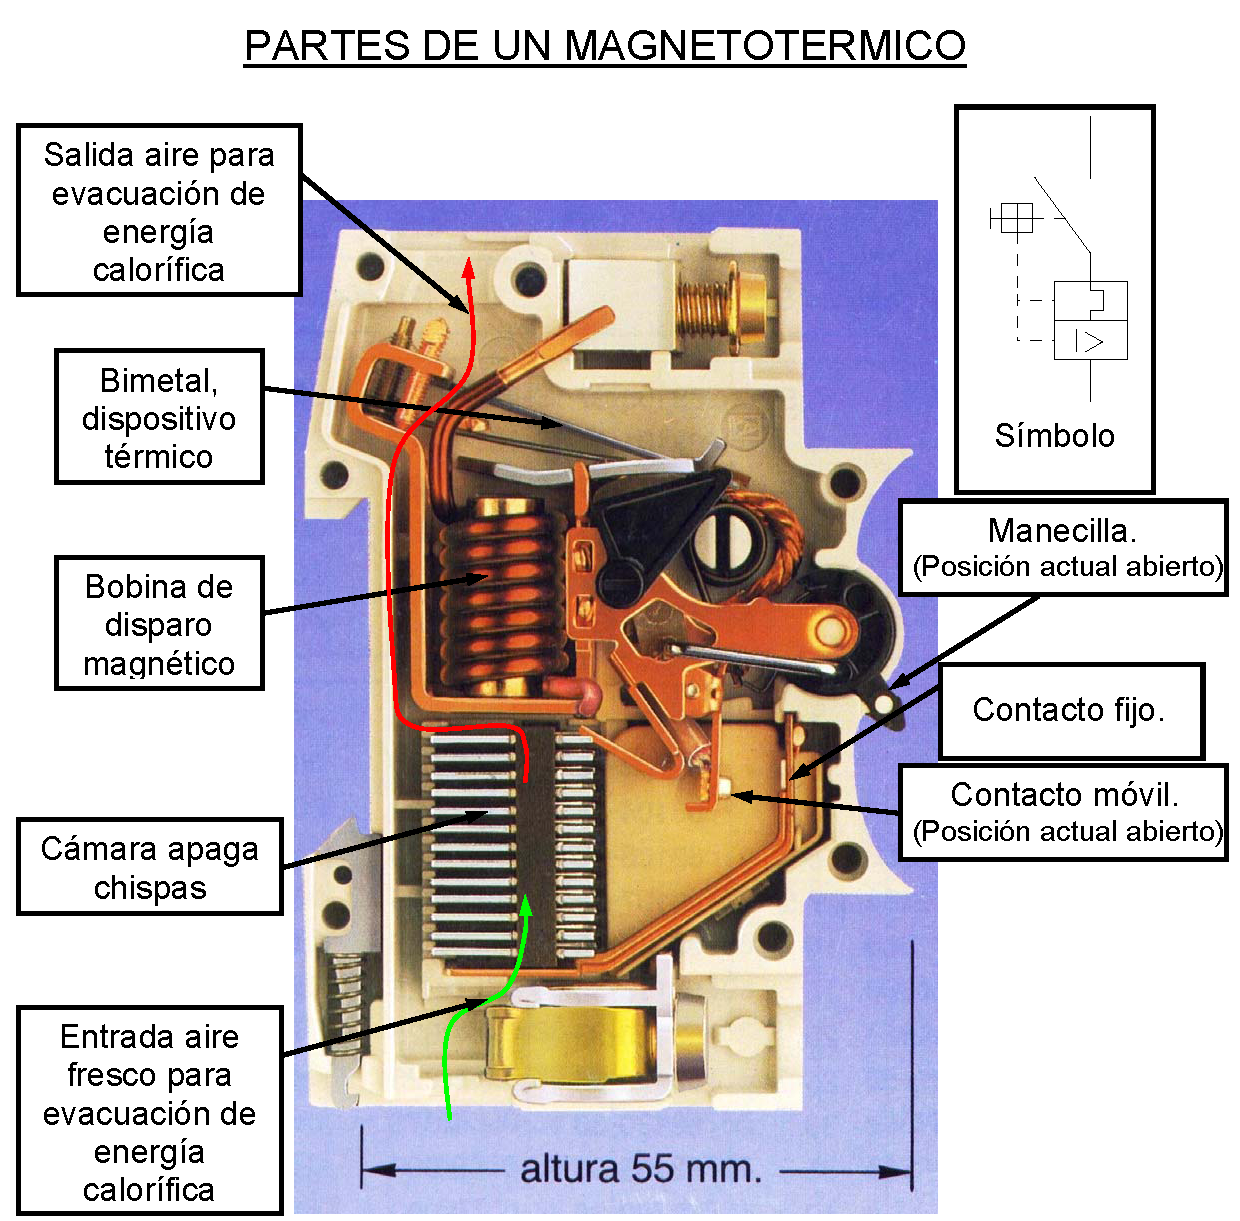
\includegraphics[height=0.8\textheight]{../figs/SeccionMagnetotermico.png}
\end{center}
\end{frame}

\begin{frame}[label={sec:orgf5b40e5}]{Interruptor diferencial}
\begin{itemize}
\item Dispositivo automático capaz de interrumpir la corriente eléctrica de un circuito cuando existe una corriente diferencial residual, indicativa de un defecto de aislamiento.
\item Para la detección emplea un transformador toroidal que abraza a todos los conductores.
\item Cuando existe un defecto, la suma fasorial de las corrientes abarcadas no será nula y, por tanto, aparecerá una intensidad en el secundario del transformador, proporcional al defecto.
\item Se emplea para la \alert{protección de las personas}.
\end{itemize}
\end{frame}

\begin{frame}[label={sec:org70045b1}]{Interruptor Diferencial}
\begin{center}
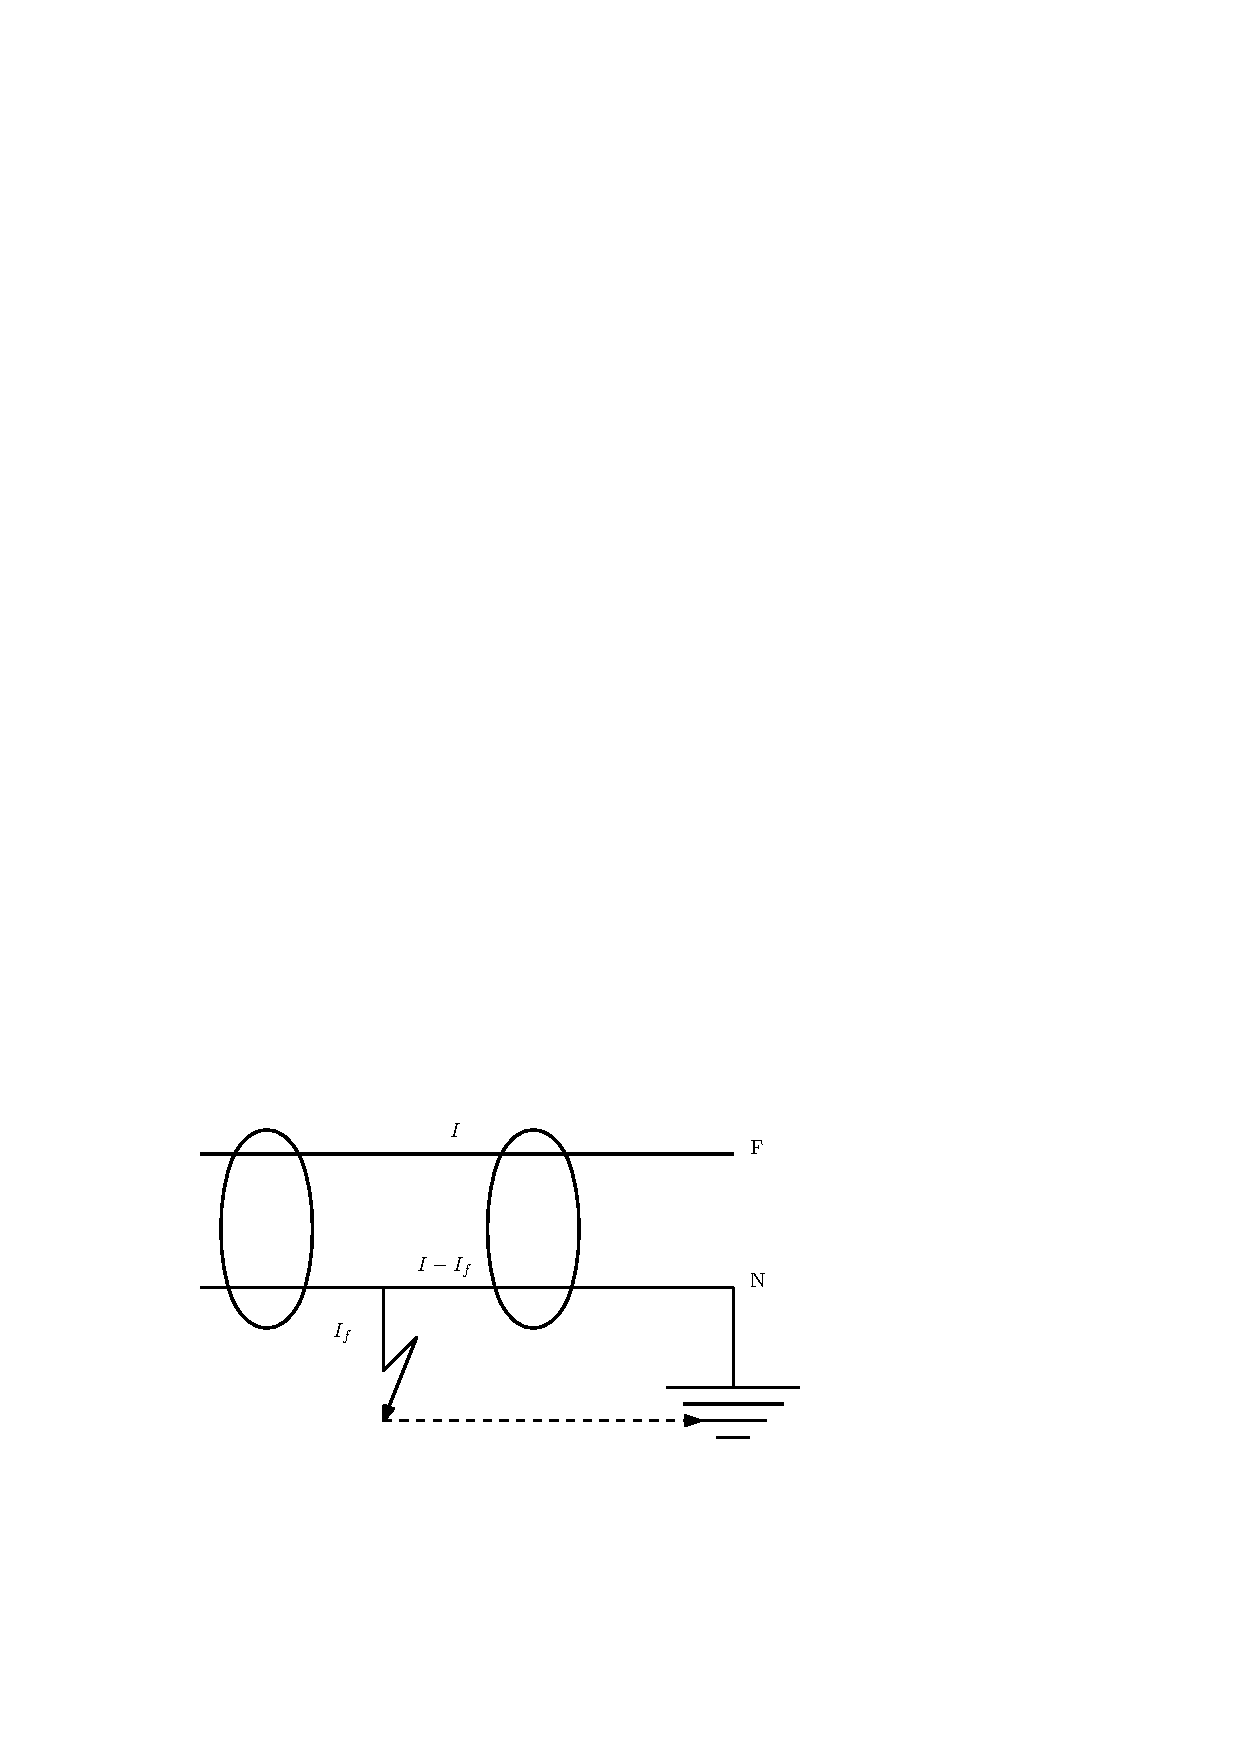
\includegraphics[height=0.3\textheight]{../figs/InterruptorDiferencial.pdf}
\end{center}

\begin{center}
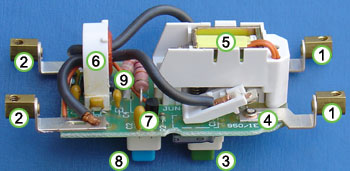
\includegraphics[height=0.3\textheight]{../figs/ResidualCurrentCircuitBreak.jpg}
\end{center}
\end{frame}

\section{Recursos}
\label{sec:org4e9072d}

\begin{frame}[label={sec:org1a0b9c5}]{Bibliografía}
\begin{itemize}
\item \alert{Fraile Mora, J.}: \emph{Máquinas Eléctricas}. Ed. Mc. Graw Hill.

\item \href{http://www.f2i2.net/legislacionseguridadindustrial/Si\_ambito.aspx?id\_am=76}{Reglamento Electrotécnico de Baja Tensión}

\item \href{https://www.schneider-electric.es/es/download/document/020511E10/}{Guía de diseño de instalaciones eléctricas (Schneider Electric)}

\item \href{http://www.directindustry.com/}{Equipos industriales}

\item \href{http://www.preoc.es/}{Base de Precios PREOC}
\end{itemize}
\end{frame}
\end{document}